% 第4章第3节：过程的构造与路径版本（逐步核构造、Kolmogorov扩张、版本与连续版本）。

\section{过程的构造与路径版本}
\label{sec:spp-construction}

前两节都假定过程已经给定。实际建模时，手中往往只有一些可以写下的规则：“从当前历史出发，下一步按某个条件分布抽取”，或者“任意有限个位置上的读数服从某个联合分布”。本节回答两个问题。第一，这些有限的规则能否拼成同一个概率空间上的一整族随机变量？有时间先后的情形用条件规律逐步构造，没有先后的情形用相容的有限维分布构造。第二，构造出来的坐标族是否具有我们想要的路径性质？上一节已经看到，连续时间下有限维分布不足以回答路径问题；我们将引入版本与不可区分这两种“相等”，并用Kolmogorov连续性准则得到连续版本。

\subsection{由条件规律逐步构造}
\label{sec:spp-kernel-construction}

\paragraph{逐步抽样的规则}
先看一个依赖整段历史的例子。罐中起初有一个标$1$的球和一个标$0$的球。每次随机摸出一个球，记下标号，把它放回，再放入一个同标号的新球。这个过程称为\term{Pólya罐}（Pólya urn）。记第$n$次的标号为$X_n$，前$n-1$次中摸到$1$的次数为$k$，此时罐中有$k+1$个$1$球、$n-k$个$0$球，于是
\[
  \mathbb P(X_n=1\mid X_1=x_1,\ldots,X_{n-1}=x_{n-1})=\frac{1+k}{n+1}.
\]
下一步的条件分布依赖全部历史中$1$的个数，而不只依赖上一步的结果。图~\ref{fig:spp-polya-tree}把前三步画成一棵树：每条边上是给定此前历史的条件概率，一条从根到叶的路径的概率是沿途条件概率的乘积。

\begin{figure}[htbp]
  \centering
  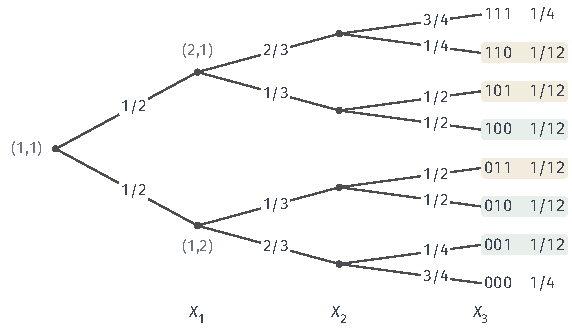
\includegraphics[width=97mm]{figures/03-optimization-evolution-and-signals/02-processes-and-trajectory-evolution/tikz/spp-polya-tree/figure.pdf}
  \caption{Pólya罐前三步的逐步构造。灰色数对是罐中$1$球与$0$球的个数，边上数字是给定此前历史时下一步标号的条件概率，右侧为三步路径及其概率（沿途条件概率之积）。含两个$1$的三条路径（黄底）概率都是$1/12$，含一个$1$的三条路径（绿底）也都是$1/12$：路径概率只依赖$1$的个数，不依赖出现的先后。}
  \label{fig:spp-polya-tree}
\end{figure}

一般地，设状态空间为可测空间$(E,\mathcal E)$，给定初始分布$\mu$和一列概率核$K_n$，$n\ge1$，其中$K_n$从历史空间$E^n$到$E$：输入历史$(x_0,\ldots,x_{n-1})$，输出下一状态的分布$K_n(x_0,\ldots,x_{n-1};\cdot)$。概率核要求对每个历史输出一个概率测度，并且对每个可测集$C$，$K_n(\cdot\,;C)$是历史的可测函数。前$n$步的联合分布由逐层“先抽历史、再按核抽下一步”给出：
\begin{equation}
  \begin{aligned}
  P_n(\mathrm dx_0,\ldots,\mathrm dx_n)
  &=\mu(\mathrm dx_0)\,K_1(x_0;\mathrm dx_1)\,K_2(x_0,x_1;\mathrm dx_2)\\
  &\qquad\cdots K_n(x_0,\ldots,x_{n-1};\mathrm dx_n).
  \end{aligned}
  \label{eq:spp-kernel-chain}
\end{equation}
这个记号的严格含义来自概率空间部分的核积分定理：给定空间$S$上的概率测度$\nu$与从$S$到$E$的概率核$K$，存在唯一的概率测度$\nu\otimes K$定义在$S\times E$上，使$(\nu\otimes K)(B\times C)=\int_BK(s;C)\,\nu(\mathrm ds)$。取$S=E^n$、$\nu=P_{n-1}$、$K=K_n$，就由$P_{n-1}$得到$P_n=P_{n-1}\otimes K_n$；从$P_0=\mu$出发归纳，即得式~\eqref{eq:spp-kernel-chain}。

\paragraph{相容性来自归一化}
逐步构造的有限维分布自动相容。对$B\in\mathcal E^{\otimes n}$，
\[
  P_n(B\times E)=\int_BK_n(x_0,\ldots,x_{n-1};E)\,P_{n-1}(\mathrm dx)=P_{n-1}(B),
\]
所以积掉最后一步就回到前一步的分布；这里用到的只是每个核的总质量为$1$。在任何以$P_n$为前$n+1$个坐标联合分布的过程中，$K_n(X_0,\ldots,X_{n-1};\cdot)$都是$X_n$给定历史的一个条件分布。

逐步构造覆盖了大多数离散时间模型。若$K_n(x_0,\ldots,x_{n-1};\cdot)=P(x_{n-1},\cdot)$只依赖最后一个状态，且核$P$不随$n$变化，就得到时间齐次的\term{Markov链}（Markov chain），第~\ref{chap:discrete-time-stochastic-processes}章研究它的回返与长期性质。例如两状态链从$X_0=0$出发，转移概率$P(0,\{0\})=0.9$、$P(0,\{1\})=0.1$，则$\mathbb P(X_1=0,X_2=1)=0.9\times0.1=0.09$。第~\ref{sec:spp-fdd-path-law}小节的自回归序列也是这样构造的，它的核是$K(y;\cdot)=\mathcal N(\rho y,1-\rho^2)$。Pólya罐则是核依赖整段历史的例子。

\begin{example}[Pólya罐的路径概率]
\label{ex:spp-polya-path}
推广到罐中起初有$a>0$个$1$球、$b>0$个$0$球（允许非整数，此时把个数理解为权重）。对任一长为$n$、含$k$个$1$的序列$(x_1,\ldots,x_n)$，按式~\eqref{eq:spp-kernel-chain}把沿途条件概率相乘。分母依次是$a+b,a+b+1,\ldots,a+b+n-1$，与序列无关；在摸到$1$的那些步上，分子依次是$a,a+1,\ldots,a+k-1$，在摸到$0$的那些步上依次是$b,b+1,\ldots,b+n-k-1$，次序只影响这些因子出现在哪一步，不影响乘积。记上升阶乘$c^{(j)}=c(c+1)\cdots(c+j-1)$，$c^{(0)}=1$，得到
\begin{equation}
  \mathbb P(X_1=x_1,\ldots,X_n=x_n)=\frac{a^{(k)}\,b^{(n-k)}}{(a+b)^{(n)}} .
  \label{eq:spp-polya-path}
\end{equation}
取$a=b=1$、$n=3$：$k=2$时为$1\cdot2\cdot1/(2\cdot3\cdot4)=1/12$，$k=3$时为$1\cdot2\cdot3/24=1/4$，与图~\ref{fig:spp-polya-tree}一致。路径概率只依赖$1$的个数，这一对称性将在第~\ref{sec:spp-exchangeable}节成为交换性的出发点。
\end{example}

\paragraph{可数步的过程}
式~\eqref{eq:spp-kernel-chain}给出了任意有限步的分布。但“最终被吸收”“频率收敛”这些问题涉及无穷多步，需要整条无穷序列上的一个概率测度。下面的定理保证这样的测度存在且唯一，而且不需要状态空间具有任何拓扑结构。

\begin{theorem}[Ionescu-Tulcea定理]
\label{thm:spp-ionescu-tulcea}
设$(E_n,\mathcal E_n)$，$n\ge0$，是任意可测空间，$\mu$是$E_0$上的概率测度，$K_n$是从$E_0\times\cdots\times E_{n-1}$到$E_n$的概率核，$n\ge1$。则在$\Omega=\prod_{n\ge0}E_n$及其乘积$\sigma$代数上存在唯一的概率测度$P$，使对每个$n$，前$n+1$个坐标的联合分布等于式~\eqref{eq:spp-kernel-chain}中的$P_n$。坐标过程$X_n(x)=x_n$在$P$下以$\mu$为初始分布，以$K_n$为各步的条件分布。
\end{theorem}

上述构造结论可参考文献\scite{math-kallenberg2021probability}。

唯一性已由定理~\ref{thm:spp-path-law}给出：两个这样的测度有相同的有限维分布。存在性的思路如下，可作为补充阅读。

\begin{proof}[存在性的证明思路]
对只依赖前$m+1$个坐标的柱集$A=B\times\prod_{n>m}E_n$，令$P(A)=P_m(B)$。由上面的相容性，同一个柱集换用更多坐标表示时值不变，所以$P$在柱集代数上有定义且有限可加。按Carathéodory延拓定理，只需验证：若柱集$A_1\supseteq A_2\supseteq\cdots$满足$P(A_k)\ge\varepsilon>0$，则$\bigcap_kA_k\ne\varnothing$。

设$A_k$依赖前$m_k+1$个坐标。对$n\ge0$，令$h_k^{(n)}(x_0,\ldots,x_n)$为“已知前$n+1$个坐标后$A_k$发生的条件概率”：$n\ge m_k$时它就是$A_k$的示性函数，$n<m_k$时用核$K_{n+1},\ldots,K_{m_k}$把后续坐标逐层积掉。于是
\begin{gather*}
  h_k^{(n)}(x_0,\ldots,x_n)=\int h_k^{(n+1)}(x_0,\ldots,x_n,y)\,K_{n+1}(x_0,\ldots,x_n;\mathrm dy),\\
  \int h_k^{(0)}\,\mathrm d\mu=P(A_k)\ge\varepsilon .
\end{gather*}
由$A_k$递减，$h_k^{(n)}$关于$k$递减，记极限为$g^{(n)}$。对上面两式令$k\to\infty$，被积函数取值于$[0,1]$，由控制收敛定理，$g^{(n)}$满足同样的递推，且$\int g^{(0)}\,\mathrm d\mu\ge\varepsilon$。于是存在$x_0$使$g^{(0)}(x_0)\ge\varepsilon$；而若$g^{(n)}(x_0,\ldots,x_n)\ge\varepsilon$，递推式说明存在$x_{n+1}$使$g^{(n+1)}(x_0,\ldots,x_{n+1})\ge\varepsilon$。归纳得到序列$x=(x_0,x_1,\ldots)$。对每个$k$取$n\ge m_k$，有$\mathbb I_{A_k}(x)=h_k^{(n)}(x_0,\ldots,x_n)\ge g^{(n)}(x_0,\ldots,x_n)\ge\varepsilon>0$，所以$x\in A_k$。
\end{proof}

证明中每一步只用到核的积分和总质量为$1$，从未用到$E_n$的拓扑。这与下一小节的Kolmogorov扩张定理形成对照：那里没有核可用，紧性代替了核的作用。

\paragraph{标准Borel空间上的两种描述}
反方向的问题是：给定一个序列的规律，能否把它写成“初始分布加历史条件核”？这需要每一步的条件分布能拼成概率核，即正则条件分布存在。在\term{标准Borel空间}（standard Borel space）上这总是可以做到的；标准Borel空间是指其可测结构同构于某个完备可分度量空间的Borel子集，$\mathbb R^d$、有限集和可数集都属于此类。于是在标准Borel状态空间上，“序列在$E^{\mathbb N_0}$上的规律”与“初始分布加历史条件核”是同一模型的两种等价描述，后者中的核在几乎处处意义下唯一。第~\ref{chap:discrete-time-stochastic-processes}章正是在这个意义下用转移核刻画离散时间过程。

\subsection{由相容有限维分布构造}
\label{sec:spp-kolmogorov-extension}

\paragraph{没有先后的索引}
逐步构造依赖时间顺序：先有过去，才谈得上给定过去的下一步。可是平面上的温度场、以输入位置为索引的随机函数都没有自然的先后。这时能够直接写下的是：任意有限个位置上的读数服从什么联合分布。于是问题变成第~\ref{sec:spp-fdd-path-law}小节问题的逆向版本：给定一族有限维分布，是否存在一个过程以它们为有限维分布？

为了把重排相容性吸收进记号，用索引的有限子集代替有序元组。对有限集$J\subseteq T$，记$E^J$为从$J$到$E$的函数全体，配乘积$\sigma$代数；对有限集$J\subseteq K$，记$\pi_{K,J}:E^K\to E^J$为限制映射$x\mapsto x|_J$，记$\pi_J:E^T\to E^J$为从整条路径到$J$上坐标的限制。

\begin{definition}[相容的有限维分布族]
\label{def:spp-consistent-family}
设对$T$的每个非空有限子集$J$给定$(E^J,\mathcal E^{\otimes J})$上的概率测度$\mu_J$。若对任意有限集$J\subseteq K\subseteq T$都有
\[
  \mu_K\circ\pi_{K,J}^{-1}=\mu_J ,
\]
就称$\{\mu_J\}$是相容的。
\end{definition}

用函数$x:J\to E$而不是有序元组表示坐标后，排列坐标只是换一种列举方式，不会产生新的测度，第~\ref{sec:spp-fdd-path-law}小节的两条相容关系合并为这一条。若过程$X$存在，令$\mu_J$为$(X_t)_{t\in J}$的分布，由定理~\ref{thm:spp-fdd-consistency}，这族分布必然相容。

\paragraph{相容性保证柱集概率有定义}
有了相容族，可以尝试在柱集上定义$P(\pi_J^{-1}(B))=\mu_J(B)$。困难在于同一个柱集可以用不同的坐标集表示：若$\pi_J^{-1}(B)=\pi_{J'}^{-1}(B')$，两种表示给出的值必须一样。相容性恰好保证这一点。令$K=J\cup J'$，则$\pi_{K,J}^{-1}(B)$与$\pi_{K,J'}^{-1}(B')$是同一个柱集在$K$上的底，二者相等，于是
\[
  \mu_J(B)=\mu_K\bigl(\pi_{K,J}^{-1}(B)\bigr)=\mu_K\bigl(\pi_{K,J'}^{-1}(B')\bigr)=\mu_{J'}(B').
\]
用同样的办法把有限个不相交的柱集放到共同的坐标集上，可知$P$在柱集代数上有限可加。剩下的是可数可加性，这一步需要状态空间的正则性。

\begin{theorem}[Kolmogorov扩张定理]
\label{thm:spp-kolmogorov-extension}
设$(E,\mathcal E)$是标准Borel空间，$T$是任意非空集合，$\{\mu_J\}$是相容的有限维分布族。则在$(E^T,\mathcal E^{\otimes T})$上存在唯一的概率测度$P$，使对每个有限集$J\subseteq T$都有$P\circ\pi_J^{-1}=\mu_J$。坐标过程$X_t(x)=x(t)$在$(E^T,\mathcal E^{\otimes T},P)$上以$\{\mu_J\}$为有限维分布。
\end{theorem}

上述构造结论可参考文献\scite{math-kallenberg2021probability}。

这个结论称为\term{Kolmogorov扩张定理}（Kolmogorov extension theorem）。唯一性仍由定理~\ref{thm:spp-path-law}给出。存在性的证明较长，下面只记录它的结构，作为补充阅读。

\begin{proof}[存在性的证明思路]
可以把$E$看成某个完备可分度量空间$\bar E$中的Borel子集。完备可分度量空间上的概率测度在Borel集上可以用紧子集从内部逼近，所以对每个$\mu_J$和$B\in\mathcal E^{\otimes J}$，存在紧集$C\subseteq B$使$\mu_J(B\setminus C)$任意小。设柱集$A_k=\pi_{J_k}^{-1}(B_k)$递减且$P(A_k)\ge\varepsilon>0$，不妨设$J_1\subseteq J_2\subseteq\cdots$。取紧集$C_k\subseteq B_k$使$\mu_{J_k}(B_k\setminus C_k)\le\varepsilon2^{-k-1}$，令$D_k=\bigcap_{j\le k}\pi_{J_j}^{-1}(C_j)\subseteq A_k$。由$A_k\subseteq A_j$（$j\le k$），
\[
  P(A_k\setminus D_k)\le\sum_{j\le k}P\bigl(A_j\setminus\pi_{J_j}^{-1}(C_j)\bigr)\le\frac\varepsilon2 ,
\]
故$P(D_k)\ge\varepsilon/2>0$，每个$D_k$非空。在$D_k$中各取一点$x^{(k)}$。$J=\bigcup_kJ_k$可数；对固定的$j$，$k\ge j$时$x^{(k)}|_{J_j}$都落在紧集$C_j$中。用对角线方法取子列，使其在$J$的每个坐标上收敛，极限$y$满足$y|_{J_j}\in C_j$对每个$j$成立。在$T\setminus J$上任意取值补全$y$，就得到$y\in\bigcap_kD_k\subseteq\bigcap_kA_k$。由此得到可数可加性，再用Carathéodory延拓定理。
\end{proof}

当$T=\mathbb N_0$时，两条构造路线给出同一个过程：在标准Borel空间上，相容族的每一步都可以分解出条件核，再用Ionescu-Tulcea定理拼接；反之，逐步构造的有限维分布总是相容的。

\paragraph{相容性的检查}
用这个定理构造过程时，真正需要检查的是相容性。下面两个例子分别给出成功与失败的情形。

第一个例子是高斯族。设对每个有限集$J$，$\mu_J$是均值向量为$(m(t))_{t\in J}$、协方差矩阵为$(k(s,t))_{s,t\in J}$的高斯分布，其中$m$与$k$是$T$上和$T\times T$上的固定函数。限制映射$\pi_{K,J}$只是删去部分坐标，是线性映射；高斯向量在线性映射下仍是高斯向量，删去坐标后的均值与协方差就是原来的子向量与子矩阵。所以只要每个$\mu_J$都是合法的高斯分布，这一族就自动相容。第~\ref{sec:spp-gaussian-processes}节将说明，“合法”恰好要求$k$半正定。

第二个例子说明，只检查低维分布之间的相容并不够。

\begin{example}[两两相容却不存在的三元规律]
\label{ex:spp-inconsistent-pairs}
取$T=\{1,2,3\}$。要求每个$X_t\sim\mathcal N(0,1)$，每一对$(X_s,X_t)$，$s\ne t$，服从相关系数为$-1$的二元高斯分布。每个二元分布的两个边缘都是$\mathcal N(0,1)$，与一元分布相容。但不存在三元分布与这三个二元分布相容：相关系数$-1$意味着$X_1=-X_2$、$X_2=-X_3$几乎必然成立，于是$X_1=X_3$，与$\operatorname{Corr}(X_1,X_3)=-1$矛盾。用矩阵语言说，所要求的协方差矩阵
\[
  \begin{pmatrix}1&-1&-1\\-1&1&-1\\-1&-1&1\end{pmatrix}
\]
对向量$(1,1,1)^\top$给出二次型$3-6=-3$，即“$\operatorname{Var}(X_1+X_2+X_3)=-3$”，不可能成立。所以相容族必须对每个有限子集都给出真正的概率测度，包括这里缺少的三元分布；低维规律彼此一致，不保证存在一个高维规律同时以它们为边缘。
\end{example}

\paragraph{扩张定理给出什么、不给出什么}
Kolmogorov扩张定理交付的是乘积可测空间$(E^T,\mathcal E^{\otimes T})$上的一个概率测度。由定理~\ref{thm:spp-countable-coordinates}，它只回答由可数个坐标决定的事件的概率。对$T=[0,1]$，它不回答路径是否连续、全程上确界多大，因为这些事件不在乘积$\sigma$代数中；对Brownian运动所要求的有限维分布，扩张定理给出的坐标过程在$\mathbb R^{[0,1]}$上有定义，却无从谈论“几乎所有路径连续”。

另一项常常需要的性质是联合可测性：要把$\int_0^tX_s\,\mathrm ds$当作随机变量，或交换时间积分与期望，需要$(s,\omega)\mapsto X_s(\omega)$关于乘积$\sigma$代数可测，而逐个时刻的可测性并不蕴含这一点。路径正则性可以补上这一缺口。

\begin{theorem}[右连续路径的联合可测性]
\label{thm:spp-joint-measurability}
设$X=(X_t)_{t\ge0}$取值于$\mathbb R^d$，且每条样本路径都右连续。则映射$(t,\omega)\mapsto X_t(\omega)$关于$\mathcal B([0,\infty))\otimes\mathcal F$可测。
\end{theorem}

\begin{proof}
对$n\ge1$，令
\[
  X^{(n)}_t(\omega)=\sum_{k=0}^\infty\mathbb I_{[k2^{-n},(k+1)2^{-n})}(t)\,X_{(k+1)2^{-n}}(\omega),
\]
即在每个二进小区间上取右端点的值。每一项是$t$的Borel函数与$\omega$的可测函数之积，关于乘积$\sigma$代数可测；对固定的$(t,\omega)$只有一项非零，所以$X^{(n)}$可测。$t$所在小区间的右端点从右侧趋于$t$，由右连续性，$X^{(n)}_t(\omega)\to X_t(\omega)$对每个$(t,\omega)$成立。可测函数的逐点极限可测。
\end{proof}

于是问题集中到一点：能否从有限维分布出发，得到一个路径右连续甚至连续、同时保持有限维分布不变的过程？这需要先说明两个过程在什么意义下算作“同一个”。

\subsection{修改、不可区分与连续版本}
\label{sec:spp-versions}

\paragraph{两种“相等”}
比较两个过程$X,Y$（定义在同一概率空间、具有相同索引集和状态空间）时，可以逐个时刻比较，也可以整条路径比较。

\begin{definition}[版本与不可区分]
\label{def:spp-modification}
若对每个$t\in T$都有$\mathbb P(X_t=Y_t)=1$，就称$Y$是$X$的一个\term{版本}（modification），也称修改。若存在零概率事件$N$，使对每个$\omega\notin N$和每个$t\in T$都有$X_t(\omega)=Y_t(\omega)$，就称$X$与$Y$\term{不可区分}（indistinguishable）。
\end{definition}

两个定义的差别在于量词的位置。版本要求“对每个$t$，几乎必然相等”，例外的零概率事件可以随$t$变化；不可区分要求“几乎必然，对所有$t$相等”，只允许一个公共的例外事件。不可区分蕴含互为版本。互为版本的过程具有相同的有限维分布：对$t_1,\ldots,t_m$，两个随机向量$(X_{t_i})_i$与$(Y_{t_i})_i$只在$\bigcup_{i\le m}\{X_{t_i}\ne Y_{t_i}\}$上不同，这是有限个零概率事件的并。由定理~\ref{thm:spp-path-law}，它们的路径规律也相同。

\paragraph{随机位置的尖点}
索引不可数时，两种相等确实不同。

\begin{example}[随机位置的尖点]
\label{ex:spp-spike}
设$U$服从$[0,1]$上的均匀分布，在$T=[0,1]$上令
\[
  X_t=\mathbb I_{\{t=U\}},\qquad Y_t=0 .
\]
对每个固定的$t$，$\mathbb P(X_t\ne Y_t)=\mathbb P(U=t)=0$，所以$X$是$Y$的版本，两者的有限维分布都是零向量的点质量。但对每个$\omega$，$X$的路径都在$t=U(\omega)$处跳到$1$：$\sup_tX_t=1$，$\sup_tY_t=0$；$Y$的每条路径连续，$X$的每条路径都不连续。图~\ref{fig:spp-spike}画出五次实现：固定任何一个时刻$t_0$，五条路径都取$0$；但每条路径都在自己的随机位置有一个尖点。
\end{example}

\begin{figure}[htbp]
  \centering
  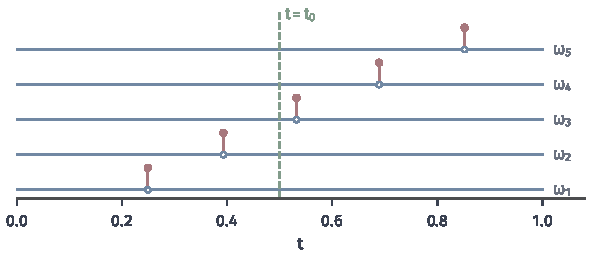
\includegraphics[width=100mm]{figures/03-optimization-evolution-and-signals/02-processes-and-trajectory-evolution/matplotlib/spp-spike/figure.pdf}
  \caption{随机位置的尖点$X_t=\mathbb I_{\{t=U\}}$，$U\sim\mathrm{Unif}(0,1)$。五行是五次独立实现（固定随机种子，纵向错开排列），每行蓝线取值$0$，红点为$t=U$处的取值$1$，空心点表示该处不取$0$。绿色虚线固定时刻$t_0=0.5$：在任何固定时刻，几乎所有实现都取$0$，与零过程无法区分；但每条路径都不连续。}
  \label{fig:spp-spike}
\end{figure}

这个例子直接回答了上一节末尾的问题：$X$与$Y$有相同的有限维分布，一个路径处处连续，一个路径处处有间断。所以有限维分布不能决定路径是否连续，“由有限维分布构造出的过程是否连续”这个问题本身就不恰当；恰当的问题是“它是否有一个连续的版本”。

索引可数时不会出现这种分歧：若$T$可数且$Y$是$X$的版本，则$N=\bigcup_{t\in T}\{X_t\ne Y_t\}$是可数个零概率事件的并，仍为零概率事件，$X$与$Y$不可区分。离散时间过程因此不必区分这两种相等。

\paragraph{右连续版本的比较}
连续时间中，路径正则性可以让可数个时刻代替全部时刻。

\begin{theorem}[右连续版本的唯一性]
\label{thm:spp-right-continuous-versions}
设$T=[0,\infty)$，过程$X,Y$取值于$\mathbb R^d$，$Y$是$X$的版本，并且存在零概率事件$N_0$，使$\omega\notin N_0$时$X$与$Y$的路径都右连续。则$X$与$Y$不可区分。
\end{theorem}

\begin{proof}
令$\mathbb Q_+=\mathbb Q\cap[0,\infty)$，$N=N_0\cup\bigcup_{q\in\mathbb Q_+}\{X_q\ne Y_q\}$。这是可数个零概率事件的并，$\mathbb P(N)=0$。对$\omega\notin N$与任意$t\ge0$，取有理数$q_k\downarrow t$，由右连续性
\[
  X_t(\omega)=\lim_{k\to\infty}X_{q_k}(\omega)=\lim_{k\to\infty}Y_{q_k}(\omega)=Y_t(\omega).
\]
所以在$N$之外两条路径处处相等。
\end{proof}

尖点例子中$X$的路径在$U$处不是右连续的（取值$1$，右侧紧邻处取$0$），所以与定理不矛盾。定理的一个直接推论是：一个过程若有连续版本，这个连续版本在不可区分的意义下唯一。于是，说“过程$X$的连续版本具有某种路径性质”是有确切含义的。

\paragraph{Hölder连续性}
在给出连续版本的判据之前，先约定一种刻画路径粗糙程度的尺度。设$0<\gamma\le1$，函数$x:[0,1]\to\mathbb R^d$若存在常数$C$使
\[
  |x(t)-x(s)|\le C|t-s|^\gamma,\qquad s,t\in[0,1],
\]
就称$x$是$\gamma$阶\term{Hölder连续}（Hölder continuous）的。$\gamma=1$是Lipschitz条件；$\gamma$越小，允许的短程变化越剧烈。例如$\sqrt t$满足$|\sqrt t-\sqrt s|\le|t-s|^{1/2}$，却在零点附近斜率无界，不是Lipschitz的。想象把路径的一小段放大：若时间放大$2$倍，高度最多放大$2^\gamma$倍。对随机路径，常数$C$可以依赖具体的实现$\omega$。

\paragraph{Kolmogorov连续性准则}
要找连续版本，需要同时控制所有短时间增量。下面的准则只要求一个关于增量矩的不等式，就能给出连续版本，并且附带Hölder指数。

\begin{theorem}[Kolmogorov连续性准则]
\label{thm:spp-kolmogorov-continuity}
设$X=(X_t)_{t\in[0,1]}$取值于$\mathbb R^d$。若存在常数$p>0$、$\beta>0$、$C<\infty$，使
\begin{equation}
  \mathbb E|X_t-X_s|^p\le C|t-s|^{1+\beta},\qquad s,t\in[0,1],
  \label{eq:spp-kolmogorov-moment}
\end{equation}
则$X$有一个路径连续的版本$\tilde X$；并且对每个$\gamma\in(0,\beta/p)$，$\tilde X$的几乎所有路径都是$\gamma$阶Hölder连续的。
\end{theorem}

这一结论称为\term{Kolmogorov连续性准则}（Kolmogorov continuity criterion）。证明的想法是先在二进有理点上逐层控制相邻点的增量，再把一般两点之间的增量拆成每层至多一步的链。证明用到Markov不等式和Borel--Cantelli引理：若一列事件的概率之和有限，则几乎必然只有有限个事件发生；它们可参考\BookChapterRef{chap:random-variable-convergence}{卷二“随机变量的收敛与积分极限”章}。

\begin{proof}
固定$\gamma\in(0,\beta/p)$。记第$n$层二进点为$D_n=\{k2^{-n}:\ k=0,1,\ldots,2^n\}$，$D=\bigcup_nD_n$。

第一步，逐层控制相邻增量。令$A_n$为事件“存在$k$使$|X_{k2^{-n}}-X_{(k-1)2^{-n}}|\ge2^{-\gamma n}$”。对每个$k$用Markov不等式和条件\eqref{eq:spp-kolmogorov-moment}，再对$2^n$个$k$求和：
\[
  \mathbb P(A_n)\le2^n\cdot\frac{C\,2^{-n(1+\beta)}}{2^{-\gamma np}}=C\,2^{-n(\beta-\gamma p)} .
\]
由$\gamma p<\beta$，右边对$n$求和有限。由Borel--Cantelli引理，存在零概率事件$N$，使对$\omega\notin N$有整数$n_0(\omega)$，当$n\ge n_0(\omega)$时第$n$层所有相邻增量都小于$2^{-\gamma n}$。

第二步，把一般二进点之间的增量拆成链。固定$\omega\notin N$和$m\ge n_0(\omega)$。对$t\in D$，记$t_m=\lfloor2^mt\rfloor2^{-m}$为$t$在第$m$层左侧最近的点。$t$与$t_m$之间可以用一条链连接：从$t_m$出发，在第$m+1,m+2,\ldots$层各至多走一步相邻点，有限步后到达$t$。每一步的增量小于该层的$2^{-\gamma n}$，因此
\[
  |X_t-X_{t_m}|\le\sum_{n>m}2^{-\gamma n}=\frac{2^{-\gamma(m+1)}}{1-2^{-\gamma}} .
\]
若$s,t\in D$且$|t-s|\le2^{-m}$，则$s_m,t_m$相同或在第$m$层相邻，$|X_{t_m}-X_{s_m}|<2^{-\gamma m}$。三段相加得
\[
  |X_t-X_s|\le c_\gamma\,2^{-\gamma m},\qquad c_\gamma=1+\frac{2\cdot2^{-\gamma}}{1-2^{-\gamma}} .
\]
对$s,t\in D$，$0<|t-s|\le2^{-n_0}$，取$m\ge n_0$使$2^{-m-1}<|t-s|\le2^{-m}$，就得到$|X_t-X_s|\le c_\gamma2^\gamma|t-s|^\gamma$。距离大于$2^{-n_0}$的两点可以用不超过$2^{n_0}$段短距离的链连接，所以$X$限制在$D$上是$\gamma$阶Hölder连续的，常数依赖$\omega$。

第三步，延拓并验证是版本。对$\omega\notin N$，$X_\cdot(\omega)$在稠密集$D$上一致连续，因而对每个$t\in[0,1]$，极限$\tilde X_t(\omega)=\lim_{s\to t,\,s\in D}X_s(\omega)$存在，所得函数$\tilde X_\cdot(\omega)$连续，并保持同样的Hölder估计；对$\omega\in N$令$\tilde X_t(\omega)=0$。每个$\tilde X_t$是可测函数的逐点极限，因而可测。最后固定$t$，取$s_k\in D$，$s_k\to t$。由条件\eqref{eq:spp-kolmogorov-moment}和Markov不等式，$\mathbb P(|X_{s_k}-X_t|>\delta)\le C|s_k-t|^{1+\beta}/\delta^p\to0$，即$X_{s_k}$依概率收敛到$X_t$；同时$X_{s_k}$几乎必然收敛到$\tilde X_t$。依概率收敛的极限几乎必然唯一，所以$\tilde X_t=X_t$几乎必然成立。

上面对固定的$\gamma$证明了Hölder性。取一列$\gamma_j\uparrow\beta/p$，对每个$\gamma_j$得到一个零概率例外事件，它们的并仍是零概率事件；由于连续版本在不可区分意义下唯一，这些$\tilde X$可以取为同一个过程。
\end{proof}

指数中的“$1+\beta$”不能换成$1$。图~\ref{fig:spp-increment-moments}比较了两个过程的增量矩。对Brownian运动，增量$B_{t+h}-B_t\sim\mathcal N(0,h)$，二阶矩为$h$，四阶矩为$3h^2$；取$p=4$、$\beta=1$，准则给出连续版本，且路径是任意$\gamma<1/4$阶Hölder连续的。更一般地，高斯变量的$2r$阶矩为$(2r-1)!!\,h^r$，取$p=2r$、$\beta=r-1$，得到任意$\gamma<(r-1)/(2r)$，令$r\to\infty$即任意$\gamma<1/2$。对速率$\lambda$的Poisson计数过程，$N_{t+h}-N_t$取非负整数值，对任意$p>0$都有
\[
  \mathbb E|N_{t+h}-N_t|^p\ge\mathbb P(N_{t+h}-N_t\ge1)=1-e^{-\lambda h},
\]
它在$h\to0$时与$\lambda h$同阶，指数只能是$1$。准则不适用，这与计数路径必然跳跃相一致。图中两条二阶矩曲线几乎重合，说明只看二阶矩无法区分“连续而粗糙”与“偶尔跳跃”；四阶矩的斜率才把两者分开。准则只是充分条件，不满足它的过程也可能有连续版本。

\begin{figure}[htbp]
  \centering
  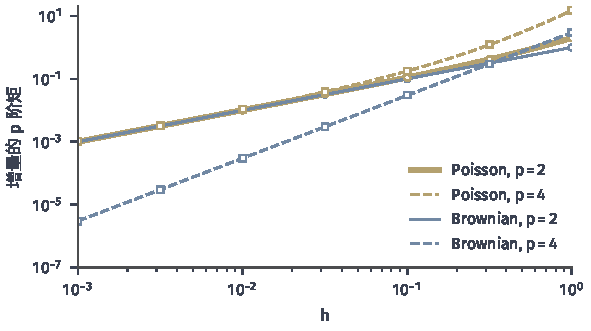
\includegraphics[width=100mm]{figures/03-optimization-evolution-and-signals/02-processes-and-trajectory-evolution/matplotlib/spp-increment-moments/figure.pdf}
  \caption{增量的$p$阶矩$\mathbb E|X_{t+h}-X_t|^p$随时间间隔$h$的变化（双对数坐标）。曲线为精确值：Brownian运动$p=2$为$h$，$p=4$为$3h^2$；速率$1$的Poisson计数过程$p=2$为$h+h^2$，$p=4$为$h+7h^2+6h^3+h^4$。空心点为每个$h$下$200000$次独立抽样的Monte Carlo估计（固定随机种子）。Brownian的四阶矩斜率为$2$，满足Kolmogorov准则；Poisson的各阶矩在小$h$处斜率都是$1$。}
  \label{fig:spp-increment-moments}
\end{figure}

准则陈述在$[0,1]$上，平移和缩放后适用于任何紧区间。对$T=[0,\infty)$，在每个$[k,k+1]$上分别取连续版本；相邻两段在公共端点$k+1$处都几乎必然等于$X_{k+1}$，把它们拼接起来，除一个零概率事件外得到整个半轴上的连续版本。

\paragraph{路径性质与路径极限}
本小节的结论为第~\ref{chap:continuous-time-stochastic-processes}章准备了两件事。第一，Brownian运动由独立高斯增量规定有限维分布，经扩张定理得到坐标过程，再由上面的四阶矩计算取连续版本；那里将据此研究Brownian路径的性质。第二，许多连续时间模型是离散模型在步长趋零时的极限，例如缩放后的随机游走。对一列过程，每个过程分别有连续版本并不够；要得到路径层面的极限，还需要对整列过程统一地控制增量，这一条件及相应的极限定理也在那一章建立。
